\documentclass{article}

\usepackage[margin=2.5cm]{geometry}
\usepackage{upgreek}
\usepackage{amsmath}
\usepackage{minted}
\usepackage{graphicx}
\usepackage{caption}
\usepackage{subcaption}
\usepackage{mathrsfs}
\usepackage[toc,page]{appendix}

%Section style
\usepackage{etoolbox} %for configuration of sloppy
\usepackage{xcolor}


\definecolor{secnum}{RGB}{102,102,102}

\makeatletter
    \def\@seccntformat#1{\llap{\color{secnum}\csname the#1\endcsname\hskip 16pt}}
\makeatother
%end section style

\begin{document}

\begin{titlepage}
\begin{center}
    \hline \\[0.2cm]
\textsc{\Large Statistical methods for machine learning}\\[0.5cm]
\textsc{\large Assignment 2}\\[0.5cm]
    \hline
    \hline
\vspace{2 cm}
\begin{tabular}{ll}
Students: & Lasse Ahlbech Madsen \\
          & Kasper Passov\\
\end{tabular}
\end{center}
\vspace{5 cm}
% \tableofcontents
\newpage
\end{titlepage}

\section{II.1}

\subsection{II.1.1}

We implemented the LDA ourselves. The code can be seen in
Part1/Opgavei11.m. \\
On the training data we observe a 14.00 \% miss rate while on the test data
the rate is 21.05 \%.

\subsection{II.1.2}

After normalizing the data we observe the same error as on the
non-transformed data. \\ 

This is unsurprising as LDA is based on the relations of the datapoints
which is unchanged when you normalise them. Graphically a plot of the data
set would look identical except for a change of the axises.

\subsection{II.1.3}

Bayes optimal classifier is a classifier which considers every hypothesis
$h$  in the hypothesis space $Ħ$ and the probability of each of them. With
$T$ being the training set and $C$ all the possible classes it can be
described as this
\begin{equation}  
   \label{eq:boc}
   y = argmax_{c_{j}\in C} \sum_{h_i \in H} P(c_j | h_i) P(T | h_i) P(h_i)
\end{equation}
We now calculate the risk. Our output can have the following 2 cases, based 
on the outputspace Y:\\
\begin{equation*}
f(S) = \left\{ \begin{array}{l l}
    1 & \quad \mbox{if \{$s_i$\in $S: 1 \in s_i$\}}\\
    0 & \quad \mbox{otherwise} \end{array} \right.
\end{equation*}
Using the Bayer optimal classifier (\ref{eq:boc}) we get the following:
\begin{alignat*}{3}
    P(h1|C) &=.25 \qquad &&P(0|h1) = 1 \qquad &&P(1|h1) = 0\\
    P(h2|C) &=.25        &&P(0|h2) = 0        &&P(1|h2) = 1\\
    P(h3|C) &=.25        &&P(0|h3) = 0        &&P(1|h3) = 1\\
    P(h4|C) &=.25        &&P(0|h4) = 0        &&P(1|h4) = 1
\end{alignat*}
therefore,\\
\begin{align*}
    \sum_{h_i \in H}& P(1|h_i)P(h_i|C) = 0.75\\
    \sum_{h_i \in H}& P(0|h_i)P(h_i|C) = 0.25
\end{align*}
and the optimal risk is then\\
\begin{equation*}
    argmax_{c_{j}\in {0,1}} \sum_{h_i \in H} P(c_j | h_i) P(h_i|D) = 1
\end{equation*}
To calculate the risk of the probalistic classifier you have to
calculate the chance of the predicted result being incorrect. In this
case with two possible outputs, it is simply frequency of '0' times the
probability of '1' + frequency of '1' times the probability of '0'.\\
\begin{align*}
      &\mathcal{R}_s(h) = {h(0) \neq y_1} + {h(1) \neq y_1}\\
      &\Downarrow\\
      &\mathcal{R}_is(h) = 0.25 * 0.75 + 0.75 * 0.25 = 37.5 \%
\end{align*}
\newpage
\section{II.2}
All code for this section can be found in Part2/II2code.py, and should compile with the following packages installed:
\begin{itemize}
    \item matplotlib
    \item numpy
    \item scipy
    \item time
    \item math
    \item sklearn
    \item patsy
\end{itemize}

\subsection{II.2.1}

On figure \ref{fig:2scatter} we have plotted the x and t variables of the training set together with 
with the real and predicted target variables on the test set. 
\begin{figure}[h!]
    \centering
    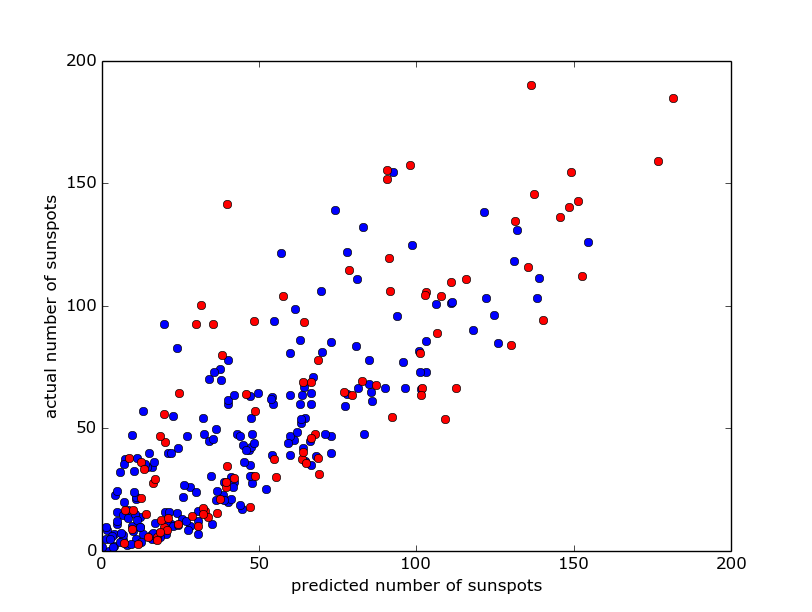
\includegraphics[width=0.5\textwidth]{Part2/II212Scatter.png}
    \caption{Selection 2 scatterplot of predicted vs actual values}
    \label{fig:2scatter}
\end{figure}\\
% x = the feature that selection 2 uses and y = the target value for each sample 
To calculate our maximum likelyhood solution We used the linear model
\begin{equation*}
    y(x, w) = w_0 + w_1 x_1 + ... + w_D x_D
\end{equation*}
and calculated the RMS using the python library sklearn. this gave us the fittings seen on 
figure \ref{fig:II21}. The plots shows number of sunspots as a function of the year.\\
It shows that Selection 3 has the best prediction, which makes sence as it has the highest dimensions.

\begin{figure}[!h]
    \centering
    \begin{subfigure}[b]{0.47\textwidth}
        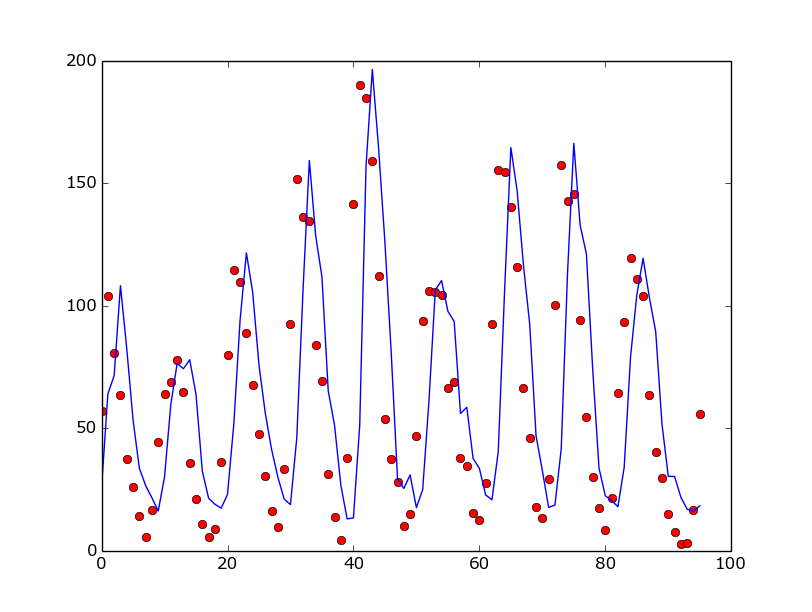
\includegraphics[width=\textwidth]{Part2/II211.png}
        \caption{Fitting with $RMS = 43.9015607236$}
    \end{subfigure}
    \begin{subfigure}[b]{0.47\textwidth}
        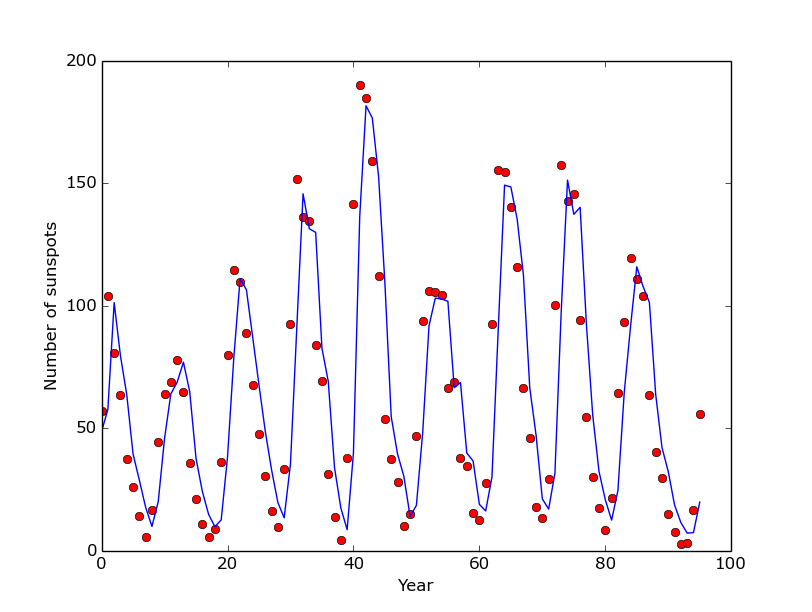
\includegraphics[width=\textwidth]{Part2/II212.png}
        \caption{Fitting with $RMS = 29.2452004653$}
    \end{subfigure}
    \begin{subfigure}[b]{0.47\textwidth}
        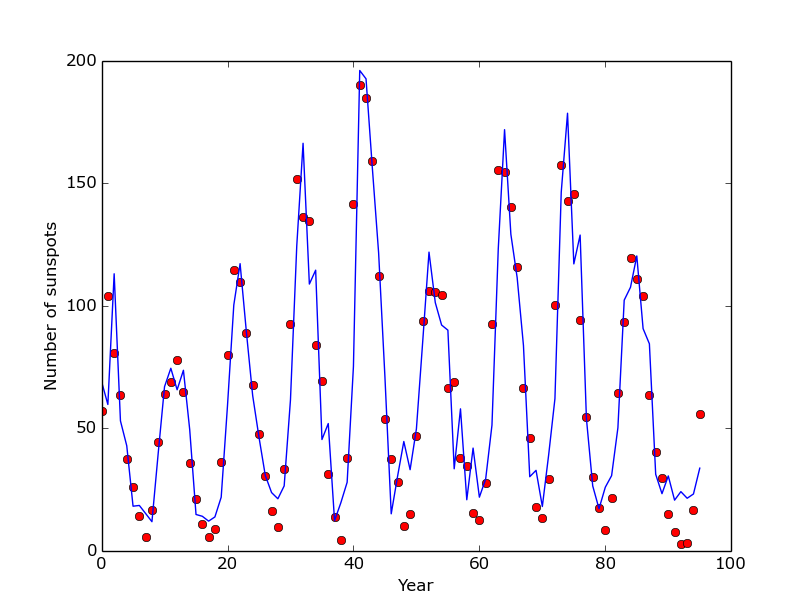
\includegraphics[width=\textwidth]{Part2/II213.png}
        \caption{Fitting with $RMS = 18.7225909686$}
    \end{subfigure}
    \caption{Fittings using linear regression and ML}
    \label{fig:II21}
\end{figure}

\subsection{II.2.2}

On figure \ref{fig:II22} the plots of our MAP estimations are shown in relation
to our ML solutions. In each picture, the blue line is the estimation of    
our Maximum likelihood solution and the red our MAP estimations given 
different values, plottet on the x-axis.\\
Please note that the alpha value is calculated by $\alpha = 10^{x} $ where x    
is plotted on the x-axis of figure \ref{fig:II22}.\\
It is easy to see, that in figure \ref{fig:II221} the ML solution is
betther than the MAP solution, as the error value from MAP 
never drops below our ML solutions rms.\\
Our MAP estimations for Selection 2 and 3 are however better then our ML solutions with the 
best values being at respectivly $x = 5.001$ with an rms of 28.6 and $x = 3.546$ with and rms of 18.57.\\
This means our \textbf{best results are Selection 3 with the MAP estimation}.
Selection 2 decents below the ML solutions at around $x \sim 3$. Selection 3 at $x \sim 2.8$

% We used the following to calculate our maximum posterior weight vector.\\
% \begin{align*}
    % p(w|\alpha) &= \mathcal{N}(w|0, \alpha^{-1}\textbf{I})\\
    % m_{N} &= \beta S_{N} \Phi^{T} \textbf{t}\\
    % S_{N} &= (\alpha \textbf{I} \cdot \beta \Phi^{T} \Phi)^{-1}
% \end{align*}
% We also know $w_{MAP} = m_N$.\\

\begin{figure}[!ht]
    \centering
    \begin{subfigure}[b]{0.4\textwidth}
        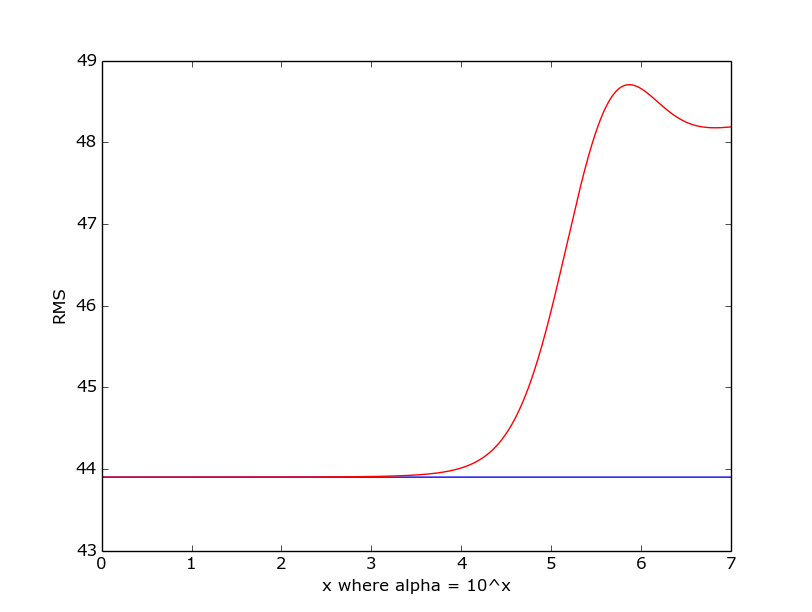
\includegraphics[width=\textwidth]{Part2/II221.png}
        \caption{Selection 1}
        \label{fig:II221}
    \end{subfigure}
    \begin{subfigure}[b]{0.4\textwidth}
        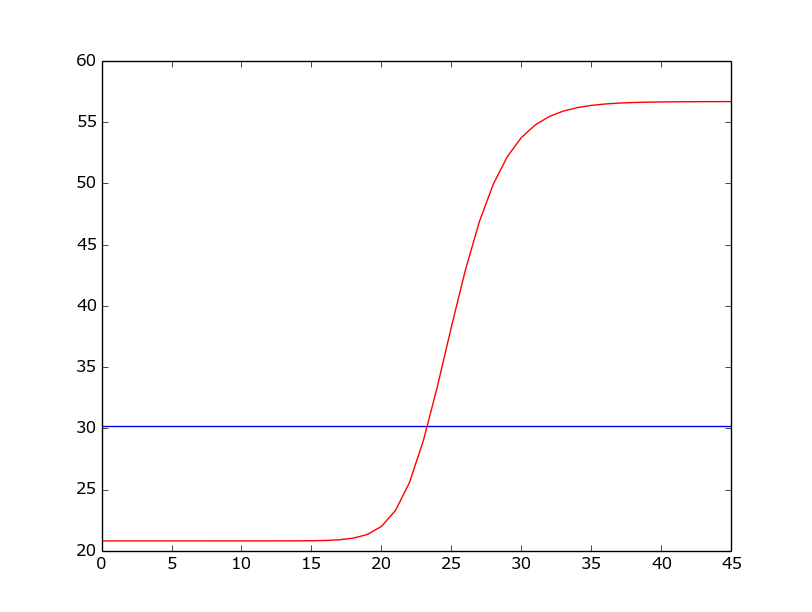
\includegraphics[width=\textwidth]{Part2/II222.png}
        \caption{Selection 2}
        \label{fig:II222}
    \end{subfigure}
    \begin{subfigure}[b]{0.4\textwidth}
        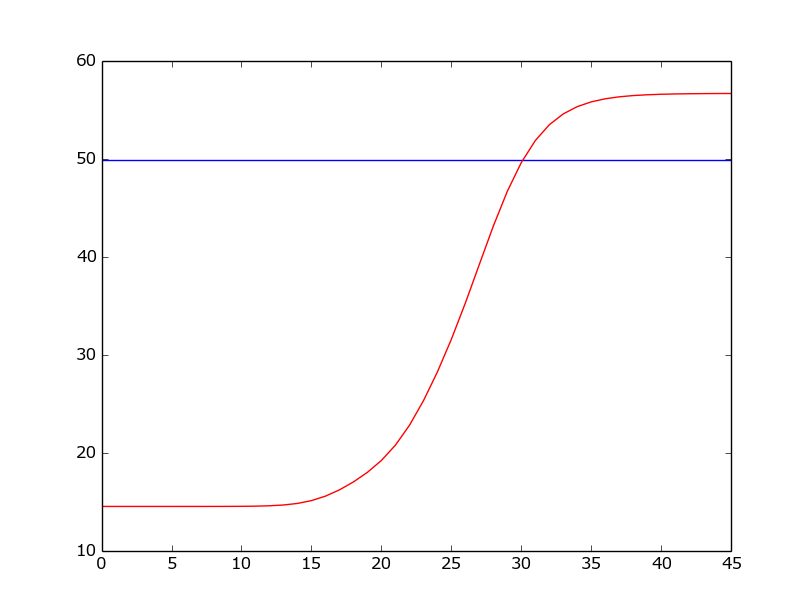
\includegraphics[width=\textwidth]{Part2/II223.png}
        \caption{Selection 3}
        \label{fig:II223}
    \end{subfigure}
    \caption{MLS vs MAP}
    \label{fig:II22}
\end{figure}

% \begin{verbatim}
% Selection 1:
% bestmN = [[-0.25979644]
          % [ 0.99404856]]
% bestrms = 43.9015675468
% bestAlpha = 1

% bestmN = [[ 0.80531681]]
% bestrms = 28.6056302671
% bestAlpha = 100230.523808

% bestmN = [[-0.02455309]
          % [ 0.20662984]
          % [-0.00638428]
          % [-0.44285572]
          % [ 1.2408648 ]]
% bestrms = 18.5789196201
% bestAlpha = 3515.60440528
% \end{verbatim}

\subsection{II.2.3}

We attempt to solve for $w$.

\begin{equation*}
    E_{D}(w) = \frac{1}{2} \sum_{n=1}^{N} r_n(t_n - w^T\phi(x_n))^2
\end{equation*}
First we differentiate the equation.

\begin{equation*}
  \frac{\delta}{\delta w} \left[ \frac{1}{2}\sum_{n=1}^{N} r_n(t_n -w^T\phi(x_n))^2 ] \right] 
\end{equation*}
We move the constants and the summation outside the derivative.

\begin{equation*}
  \frac{1}{2}\sum_{n=1}^{N} r_n \frac{\delta}{\delta w} \left[ (t_n - w^T\phi(x_n))^2 \right]
\end{equation*}
We use the chain rule and solve the two parts individually.

\begin{equation*}
    \frac{1}{2}\sum_{n=1}^{N} r_n 2(t_n - w^T\phi(x_n)) \cdot \frac{\delta}{\delta w} \left[ (t_n - w^T\phi(x_n) \right]
\end{equation*}

\begin{equation*}
    \sum_{n=1}^{N} r_n (t_n - w^T\phi(x_n)) \cdot 0 - 1 \cdot \phi(x_n)
\end{equation*}
As we want to find the stationary point we set the other side of the
equation to 0.

\begin{equation*}
    \sum_{n=1}^{N} r_n (t_n - w^T\phi(x_n)) \cdot \phi(x_n) = 0
\end{equation*}
We multiply into the parenthesis.

\begin{equation*}
    \sum_{n=1}^{N} (r_n t_n - r_n w^T\phi(x_n)) \cdot \phi(x_n)
\end{equation*}

\begin{equation*}
    \sum_{n=1}^{N} r_n t_n \phi(x_n) - r_n w^T\phi(x_n) \cdot \phi(x_n)
\end{equation*}
Then we split the sum into two parts. 

\begin{equation*}
    \sum_{n=1}^{N} r_n t_n \phi(x_n) - \sum_{n=1}^{N} r_n w^T\phi(x_n) \cdot \phi(x_n)
\end{equation*}
We introduce $R$ and set it as the matrix seen below. This allows us to
change $r_n$ to $R$ and move it outside the summation.

\begin{equation*}
    \begin{array}{r c c c c}
    &   r_1 & 0   & .. & 0   \\
    &   0   & r_2 & .. & 0   \\
  R =   &  ...  & ... & .. & ...   \\
    &   0   & 0   & .. & 0   \\
    &   0   & 0   & .. & r_N 
    \end{array}
\end{equation*}
We move $w$ and $R$ outside the two summations.

\begin{equation*}
    w^T R \sum_{n=1}^{N} \phi(x_n)^2 - R \sum_{n=1}^{N} t_n \phi(x_n) 
\end{equation*}
Seeing as $\phi(x_n)$ is basically a row of a designmatrix, we can view it
as a design matrix $\Phi$ outside the summation.

\begin{equation*}
    \begin{array}{r c c c c}
        &  \phi_0(x_1) & \phi_1(x_1)   & .. & \phi_{M-1}(x_1) \\
        &  \phi_0(x_2) & \phi_1(x_2)   & .. & \phi_{M-1}(x_2) \\
  \Phi =   &  ...  & ... & .. & ...   \\
           &  \phi_0(x_{N-1}) & \phi_1(x_{N-1})   & .. & \phi_{M-1}(x_{N-1}) \\
        &  \phi_0(x_N) & \phi_1(x_N)   & .. & \phi_{M-1}(x_N) 
    \end{array}
\end{equation*}
$t_n$ is a vector outside the summation and can be freely moved as well
and the summations are done away with. 

\begin{equation*}
  0 = w^T R (\Phi^T \Phi) - R \bar{t}^T \Phi 
\end{equation*}
Now all that remains is to isolate $w$.

\begin{equation*}
  w^T R (\Phi^T \Phi) = R \bar{t} \Phi 
\end{equation*}
We can move $w$ to the right on left handside and transpose parenthesis in
its stead. And since it contains a matrix multiplied with its transpose we
can drop it. On the right hand side we observe that we can move $t$ to the
other side of $\Phi$ if we transpose it instead. 

\begin{equation*}
  R (\Phi^T \Phi) w = R \bar{t} \Phi 
\end{equation*}
Now we can multiply both sides by the inverse of $(\Phi^T \Phi)$. Since R
is a diagonal matrix we can move that to the right of the parenthesis.

\begin{equation*}
  R w = (\Phi^T \Phi)^{-1} R \bar{t} \Phi 
\end{equation*}
And the inverse of $R$. This gives us the solution for $w$.

\begin{equation*}
  w = R^{-1}(\Phi^T \Phi)^{-1} R \bar{t} \Phi 
\end{equation*}

\subsubsection{II.2.3.I}

If we have some knowledge of the data, the weights can be adjusted to make
up for some assumed noise in the dataset.

\subsubsection{II.2.3.II} 

If we have replicate datapoints we risk
these points become overly important for our error function, when we use
weigthed sum of square we can reduce the impact of the replicated points.


\end{document}
